% Options for packages loaded elsewhere
\PassOptionsToPackage{unicode}{hyperref}
\PassOptionsToPackage{hyphens}{url}
\PassOptionsToPackage{dvipsnames,svgnames,x11names}{xcolor}
%
\documentclass[
]{report}
\usepackage{amsmath,amssymb}
\usepackage[]{inter}
\usepackage{iftex}
\ifPDFTeX
  \usepackage[T1]{fontenc}
  \usepackage[utf8]{inputenc}
  \usepackage{textcomp} % provide euro and other symbols
\else % if luatex or xetex
  \usepackage{unicode-math}
  \defaultfontfeatures{Scale=MatchLowercase}
  \defaultfontfeatures[\rmfamily]{Ligatures=TeX,Scale=1}
\fi
% Use upquote if available, for straight quotes in verbatim environments
\IfFileExists{upquote.sty}{\usepackage{upquote}}{}
\IfFileExists{microtype.sty}{% use microtype if available
  \usepackage[]{microtype}
  \UseMicrotypeSet[protrusion]{basicmath} % disable protrusion for tt fonts
}{}
\makeatletter
\@ifundefined{KOMAClassName}{% if non-KOMA class
  \IfFileExists{parskip.sty}{%
    \usepackage{parskip}
  }{% else
    \setlength{\parindent}{0pt}
    \setlength{\parskip}{6pt plus 2pt minus 1pt}}
}{% if KOMA class
  \KOMAoptions{parskip=half}}
\makeatother
\usepackage{xcolor}
\IfFileExists{xurl.sty}{\usepackage{xurl}}{} % add URL line breaks if available
\IfFileExists{bookmark.sty}{\usepackage{bookmark}}{\usepackage{hyperref}}
\hypersetup{
  pdftitle={Analyzing COVID-19 in Austin},
  pdfauthor={Matt Worthington},
  colorlinks=true,
  linkcolor={blue},
  filecolor={Maroon},
  citecolor={Blue},
  urlcolor={Blue},
  pdfcreator={LaTeX via pandoc}}
\urlstyle{same} % disable monospaced font for URLs
\usepackage[top=30mm,left=20mm,heightrounded]{geometry}
\usepackage{longtable,booktabs,array}
\usepackage{calc} % for calculating minipage widths
% Correct order of tables after \paragraph or \subparagraph
\usepackage{etoolbox}
\makeatletter
\patchcmd\longtable{\par}{\if@noskipsec\mbox{}\fi\par}{}{}
\makeatother
% Allow footnotes in longtable head/foot
\IfFileExists{footnotehyper.sty}{\usepackage{footnotehyper}}{\usepackage{footnote}}
\makesavenoteenv{longtable}
\usepackage{graphicx}
\makeatletter
\def\maxwidth{\ifdim\Gin@nat@width>\linewidth\linewidth\else\Gin@nat@width\fi}
\def\maxheight{\ifdim\Gin@nat@height>\textheight\textheight\else\Gin@nat@height\fi}
\makeatother
% Scale images if necessary, so that they will not overflow the page
% margins by default, and it is still possible to overwrite the defaults
% using explicit options in \includegraphics[width, height, ...]{}
\setkeys{Gin}{width=\maxwidth,height=\maxheight,keepaspectratio}
% Set default figure placement to htbp
\makeatletter
\def\fps@figure{htbp}
\makeatother
\setlength{\emergencystretch}{3em} % prevent overfull lines
\providecommand{\tightlist}{%
  \setlength{\itemsep}{0pt}\setlength{\parskip}{0pt}}
\setcounter{secnumdepth}{5}
% Make \paragraph and \subparagraph free-standing
\ifx\paragraph\undefined\else
  \let\oldparagraph\paragraph
  \renewcommand{\paragraph}[1]{\oldparagraph{#1}\mbox{}}
\fi
\ifx\subparagraph\undefined\else
  \let\oldsubparagraph\subparagraph
  \renewcommand{\subparagraph}[1]{\oldsubparagraph{#1}\mbox{}}
\fi
\usepackage{amsmath}
\usepackage{booktabs}
\usepackage{caption}
\usepackage{longtable}
\makeatletter
\makeatother
\makeatletter
\@ifpackageloaded{caption}{}{\usepackage{caption}}
\AtBeginDocument{%
\renewcommand*\contentsname{Table of contents}
\renewcommand*\listfigurename{List of Figures}
\renewcommand*\listtablename{List of Tables}
\renewcommand*\figurename{Figure}
\renewcommand*\tablename{Table}
}
\@ifpackageloaded{float}{}{\usepackage{float}}
\floatstyle{ruled}
\@ifundefined{c@chapter}{\newfloat{codelisting}{h}{lop}}{\newfloat{codelisting}{h}{lop}[chapter]}
\floatname{codelisting}{Listing}
\newcommand*\listoflistings{\listof{codelisting}{List of Listings}}
\makeatother
\makeatletter
\@ifpackageloaded{caption}{}{\usepackage{caption}}
\@ifpackageloaded{subcaption}{}{\usepackage{subcaption}}
\makeatother
\makeatletter
\@ifpackageloaded{tcolorbox}{}{\usepackage[many]{tcolorbox}}
\makeatother
\makeatletter
\@ifundefined{shadecolor}{\definecolor{shadecolor}{rgb}{.97, .97, .97}}
\makeatother
\makeatletter
\@ifpackageloaded{sidenotes}{}{\usepackage{sidenotes}}
\@ifpackageloaded{marginnote}{}{\usepackage{marginnote}}
\makeatother
\makeatletter
\makeatother
\ifLuaTeX
  \usepackage{selnolig}  % disable illegal ligatures
\fi

\title{Analyzing COVID-19 in Austin}
\author{Matt Worthington}
\date{08-13-2020}

\begin{document}
\maketitle

\ifdefined\Shaded\renewenvironment{Shaded}{\begin{tcolorbox}[frame hidden, interior hidden, borderline west={3pt}{0pt}{shadecolor}, enhanced, boxrule=0pt, sharp corners]}{\end{tcolorbox}}\fi

\renewcommand*\contentsname{Contents}
{
\hypersetup{linkcolor=}
\setcounter{tocdepth}{2}
\tableofcontents
}
\listoffigures
\listoftables
Approaching the six-month mark of COVID-19 in Texas, one of the more
common topics of discussion I hear is what the effects of coronavirus on
our communities reveals about the world that existed before. And where
we knew little about COVID-19 back in March, since that time a lot has
been documented about what increases the risk of not only becoming
severely ill, but also what increases the risk of being exposed to
COVID-19 before you even get sick---such as having a job that requires
you to be physically present for work (as opposed to working remotely
from home) or not having access to a reliable internet connection.

That said, I want to explore some of these things in a series of blog
posts--to see who is not only getting COVID, but also \emph{where} folks
are most at risk of being exposed to COVID and where they're most at
risk of not bouncing back. The trouble in answering these questions is
that getting good data is difficult and, once you have it, organizing
the data in a way that is useful and meaningful for others is even
harder. So, I'm going to pace myself and search for datasets that can
inform our conversation. For the purposes of these blog posts, I'm just
going to focus on looking at the city-wide data in Austin---where I
live---because I know all the data exists with regards to the questions
I have pulled together. If you have questions, I invite you to ask them
as well and I'll do my best to find data that can help provided some
meaningful insight.

\marginnote{\begin{footnotesize}

The Texas Tribune had
\href{https://www.texastribune.org/2020/08/04/texas-coronavirus-data/}{a
good write-up on the caveats of state-wide data} that I' would recommend
reading on this topic.

\end{footnotesize}}

\hypertarget{who-is-getting-covid-19-in-austin}{%
\chapter{Who is getting COVID-19 in
Austin?}\label{who-is-getting-covid-19-in-austin}}

Before we do any exploration of the more complicated questions
identified, the best starting point would be exploring where COVID is
occuring most in Austin. So let's look at that before digging into other
questions and start by pulling
\href{https://www.arcgis.com/home/item.html?id=08e581f856cb4ceaa56adf4493d77264\&sublayer=0\&view=list\&sortOrder=true\&sortField=defaultFSOrder\#overview}{Austin
Public Health's data}---which organizes cases at the zip code level and
updated frequently---to map out cases. We don't have access to where
deaths occur most often, but cases at the zip code level is more than
you can find in a lot of places. So we'll use what we have.

Here's where cases are occurring most often right now:

\begin{figure}

{\centering 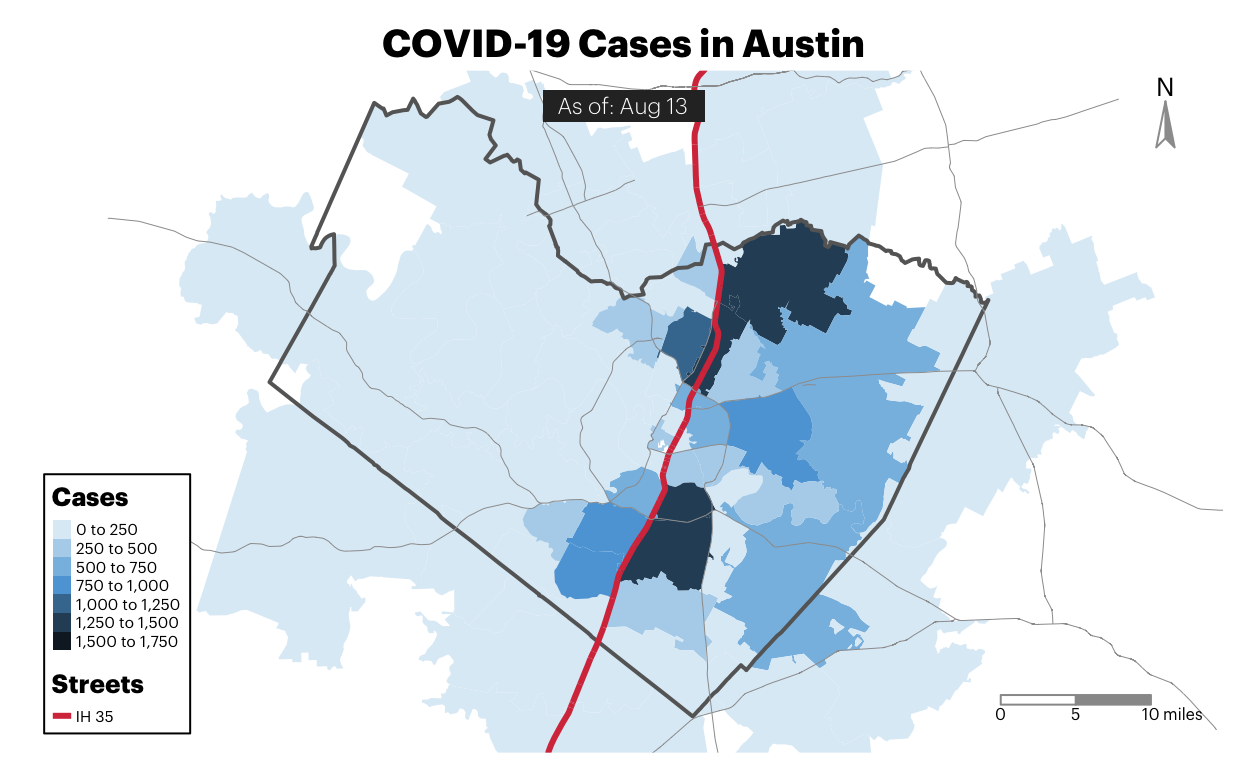
\includegraphics{covid_case_map.png}

}

\end{figure}

The first thing to notice is that cases are largely consolidated east of
I-35. Without additional context, it's worth wondering what role an
interstate plays in shielding folks on one side from Coronavirus. With
additional context about how the city was intentionally segregated
through a ``master plan'' developed in 1928 that used I-35 as a form of
physical division, it's worth paying attention to the dynamics of I-35
and including it as a geographical marker throughout future analyses.

For those unfamiliar, I would highly recommend reading through
\href{https://projects.statesman.com/news/economic-mobility/}{this
analysis by the Austin Statesman} on the role of I-35 in the city's
history of racial segregation, as a starting point. Other histories have
been documented elsewhere, but this is a good starting point.

\end{footnotesize}}

In the next few blog posts, I'll be writing about risk + resilience.
Originally, I wanted to include everything here, but the charts and
analysis became pretty extensive. For fear of exhausting everyone,
including myself. We'll take these questions piece by piece.

\textbf{Next Blogpost:} Who should be most worried about getting COVID?

\textbf{Note about this series:} If you're interested in asking specific
questions to explore in this, reach out to me via Facebook or Twitter
and I'll do my best to find data that can help provide some kind of
meaningful answer.

\textbf{Where can I find the code for this blog?} Once I clean up the
mess in this repo, I'll make it public on github. For now, I'm happy to
share individual the Rmarkdown file used to produce each article.

TLDR \textbar{} Why not do this at the statewide level?

Originally, I considered focusing these articles at the statewide level
for Texas, but I kept running into issues around finding data that could
meaningfully answer some of my questions. The reasons for this are many,
but some of the state's existing COVID-19 data cannot be aggregated at
anything beyond the statewide level for reasons outside of their
control.

\hypertarget{example---test-positivity}{%
\subsection{Example - Test Positivity}\label{example---test-positivity}}

For example, county-level test positivity is one of those things that
has been difficult because COVID-19 lab testing has largely been
decentralized, with over 97\% of tests being conducted in commercial
labs. Consequently, this means the state has to then coordinate data
from over 4 million tests conducted outside of state testing labs.

\captionsetup[table]{labelformat=empty,skip=1pt}
\setlength{\LTpost}{0mm}
\begin{longtable}{r|lr}
\caption*{
{\large \textbf{Number of People Tested for SARS-CoV-2 in Texas, By Lab Type}} \\ 
{\small Source: Texas Department of State Health Services | As of August 10th at 3:00PM CST\textsuperscript{1}}
} \\ 
\toprule
\multicolumn{1}{l}{} & \textbf{Location} & \textbf{Tests Processed} \\ 
\midrule
 & Total People Tested in Texas by Public Health Lab & $122.02K$ \\ 
 & No. Tests by Commercial labs* & $4.49M$ \\ 
\midrule 
\midrule 
Total Tests & — & $4,611,777$ \\ 
\bottomrule
\end{longtable}
\begin{minipage}{\linewidth}
\textsuperscript{1}\href{https://www.dshs.state.tx.us/coronavirus/additionaldata/}{Data: From the \textquotesingle{}Accessible Dashboard Data\textquotesingle{} File, under the \textquotesingle{}Tests\textquotesingle{} tab.}\\
*Unable to deduplicate figures for Commercial labs.\\
\end{minipage}

And given that these commercial labs aren't actually part of a state
agency, this means they have to learn new reporting rhythms and do work
that, perhaps, they didn't plan for or know they needed to do--such as
keep all of the positives and negatives for each county, record those in
a database by the county of origin, deduplicate them by the person who
got the test, and then share all of that information back to the state
in a manner that is uniform with all the other private labs in the
state.

That said, not being able to compare how much a county is testing with
how much they're testing positive weakens a potential analysis and
limits how much you can explore the dynamics between risk factors and
things like test positivity.

\hypertarget{example---demographic-data}{%
\subsection{Example - Demographic
Data}\label{example---demographic-data}}

Another example of this information is demographic data about cases and
fatalities. That information also doesn't exist broken down by
county--sometimes due to HIPAA requirements.

So if you wanted to analyze geographic COVID-19 trends between counties
across multiple pieces of data such as demographic, known risk-factors,
and other trends, you'd have a hard time accomplishing that because it
currently doesn't exist.

For that reason, I've chosen to just focus on using city-level data
given that cities tend to have better access to local information about
their communities.

\hypertarget{photo-credit}{%
\chapter{Photo Credit}\label{photo-credit}}

Photo by Ryan Magsino on Unsplash

\end{document}
